\documentclass[10pt,a4paper]{article}
\usepackage[T1]{fontenc}
\usepackage[utf8]{inputenc}
\usepackage{lmodern}
\usepackage[margin=24mm,top=22mm,bottom=23mm]{geometry}
\usepackage{amsmath,amssymb,graphicx,booktabs,longtable,array,xcolor,calc}
\usepackage[font=small,labelfont=bf]{caption}
\usepackage{hyperref}
\hypersetup{colorlinks=true,linkcolor=blue!45!black,urlcolor=blue!45!black,pdftitle={PRAgent:
AI-Assisted Physics Paper Reproduction}}
\urlstyle{same}
\providecommand{\tightlist}{\setlength{\itemsep}{0pt}\setlength{\parskip}{0pt}}
\providecommand{\pandocbounded}[1]{#1}
\setlength{\emergencystretch}{4em}
\setlength{\parindent}{0pt}
\setlength{\parskip}{4pt}
\linespread{1.01}
\setcounter{secnumdepth}{2}
\renewcommand{\topfraction}{0.93}
\renewcommand{\bottomfraction}{0.87}
\renewcommand{\textfraction}{0.07}
\renewcommand{\floatpagefraction}{0.75}
\widowpenalty=10000
\clubpenalty=10000
\begin{document}
\begin{center}
{\LARGE\bfseries PRAgent: AI-Assisted Physics Paper Reproduction\par}
\vspace{6pt}
{\large Capabilities and Evidence from a 100-Paper Project\par}
\vspace{8pt}
% Author names, order and affiliation are awaiting author-provided metadata.
% Do not submit this file without completing the author block.
{\small Technical report draft; author metadata pending\par}
\vspace{5pt}

{\small September 2026\par}
\end{center}
\begin{abstract}
PRAgent connects physics-paper interpretation, numerical implementation and scientific assessment in a human-guided research workflow. We examine the system through public implementations and a documentary audit of a fixed 100-paper project. Three cases provide concrete evidence: resource-bound code that refines large integer decisions with 60-digit arithmetic; quantum dynamics implemented in conserved particle sectors; and finite-ensemble discord calculations that expose a discrepancy with an analytical reference. A surface-code case illustrates a system-level distinction: checks pass for an implemented repetition-code proxy, while the original paper target remains unaccepted. To evaluate the breadth of these results, we trace 3,241 archived result-object records from 95 papers to their declared comparison conditions and references, and reconcile summary and detailed assessment records. This audit finds that the 26 papers with all associated checks historically labelled reproduced and the 26 with summary-level review marked passed are disjoint. Consequently, check-label fractions cannot serve as a scientific reproduction rate. The contribution is an inspectable implementation and assessment workflow, supported by numerical examples and explicit evidence links. The archive establishes bounded capabilities within that workflow; it does not yet establish an autonomous-agent success rate or complete reproduction of the cohort.

\end{abstract}

\section{Introduction}\label{introduction}

A physics paper specifies a scientific argument, but rarely a complete
software task. Reproducing it requires decisions about notation,
state-space representation, numerical precision, observables and
comparison conditions. A program can run successfully while computing a
different model or testing a weaker claim. A useful scientific agent
must therefore connect implementation to the physical question and make
that connection available for inspection.

PRAgent is an AI-assisted system for this work. It organizes paper
interpretation, numerical implementation and assessment around a
persistent research case. Its public output, distributed through
RunThePaper, includes derivations, case-specific code, generated arrays
and explanations of what the calculation establishes. The system is used
with human guidance; throughout this report, demonstrated capability
refers to what is implemented and evidenced in that combined workflow.

We make these capabilities assessable through source-target-to-evidence
chains. Three detailed cases supply the numerical examples.
Hamiltonian-simulation resource estimates require stable arithmetic and
precision-aware integer decisions. Quantum walks use conserved particle
sectors to construct exact finite-dimensional dynamics. Quantum-discord
calculations distinguish finite ensembles from an analytical reference
and from an unpublished author realization. A further case shows how the
assessment records distinguish local model checks from acceptance of the
source target. A uniform documentary audit then tests whether aggregate
labels across the fixed 100-paper project can support a broader
performance claim. The technical contribution is the implemented
research system and its inspectable evidence across these tasks; the
source papers supply the underlying physical methods.

\section{Research context}\label{research-context}

Traceable computation and accessible research materials are central to
computational reproducibility {[}1,2{]}. They motivate PRAgent's
persistent case structure: a numerical figure should be connected to
equations, inputs, implementation and checks. This also provides a way
to evaluate an agent's scientific work through the objects it produces.

PaperBench, CORE-Bench and MLE-bench evaluate complementary forms of
research replication and computational engineering {[}3--5{]}. The
present report is a capability study of a system used across
heterogeneous physics tasks. It examines implemented methods and their
evidence; comparative performance under matched budgets remains an
experimental question. The detailed physical examples implement qDRIFT
resource formulas, a quantum-walk model and DQC1 discord calculations
from their respective source papers {[}6--8{]}.

\section{PRAgent capabilities and system
design}\label{pragent-capabilities-and-system-design}

\subsection{Connecting the scientific task to executable
code}\label{connecting-the-scientific-task-to-executable-code}

A PRAgent research case records the paper identity, scientific scope,
equations, configuration, implementation, generated outputs and
assessment. A source object identifies a curve, table entry or
analytical statement. An execution target specifies the computation that
addresses it. Artifacts preserve the resulting arrays, diagnostics and
explanation. One propagation can support several observables, while one
plotted result may require several convergence checks; these
relationships remain explicit in the case.

The numerical task fixes the model, observable, system size, parameters,
boundary conditions and approximation regime. Equation records connect
the source expressions to the functions and configuration fields that
implement them. This connection is where the case-specific physics
enters: a conserved sector can define an exact basis, a resource
estimate can require inequality evaluation, and an ensemble study must
specify which distribution is sampled.

\subsection{Implementing and checking the
calculation}\label{implementing-and-checking-the-calculation}

Case implementations separate model construction, solution, observables
and rendering. This allows generated numerical tables to be inspected
independently of the plot, and lets several observables share one solver
output. Checks are tied to the scientific object: conservation for
dynamics, neighboring integer inequalities for resource bounds, and
sampling intervals for an ensemble. Control calculations test the
consequences of changing a physical assumption.

The workflow in Fig. 1 connects these computations to assessment and
revision. PRAgent retains the target, configuration and evidence
associated with each result, including unresolved comparisons. This
supports targeted follow-up: revise the model, investigate a convention,
extend a calculation or obtain a missing input. The scientific meaning
of a check is preserved alongside its pass or fail status.

\begin{center}
\begin{minipage}{\linewidth}
\centering
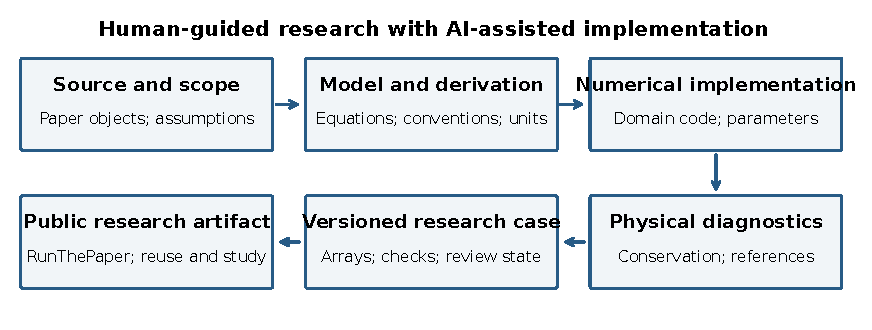
\includegraphics[width=0.80\linewidth]{figures/fig1_workflow.pdf}
\captionof{figure}{PRAgent's human-guided research workflow. Paper interpretation, numerical implementation and assessment produce a persistent research case. Human guidance can shape the task and revisions; case-specific code performs the numerical work. Derivations, arrays and review records remain linked to the result, and selected artifacts enter the public RunThePaper collection. Dashed connections indicate human guidance; solid arrows indicate workflow or artifact transfer.}
\end{minipage}
\end{center}

\subsection{A concrete assessment chain: a valid proxy is an incomplete
target}\label{a-concrete-assessment-chain-a-valid-proxy-is-an-incomplete-target}

Case \texttt{2502.20558}, target T001, makes the assessment model
tangible. The source target is the logical-error-versus-rounds
comparison in Fig. 2b for surface-code memory with delayed-erasure
handling and maximum-likelihood decoding. The public implementation
instead computes a classical repetition-code analogue. Table 1 follows
the links preserved in the frozen archive.

\begin{center}
\begin{minipage}{\linewidth}
\small
\renewcommand{\arraystretch}{1.15}
\captionof{table}{A frozen cross-artifact assessment chain. Exact fields, source pointers and file-presence checks are supplied in \texttt{anc/audit\_system\_chain.json}.}
\begin{tabular}{@{}p{0.20\linewidth}p{0.37\linewidth}p{0.36\linewidth}@{}}
\toprule
Evidence layer & Observed record & Meaning for the source target \\
\midrule
Source objects & Three Fig. 2b items: exact-time, no-SSR and SSR curves & The requested observable belongs to the surface-code method. \\
Implemented calculation & Repetition-code proxy; distance 5, loss probability 0.01, 200,000 shots & An executable mechanism model is available. \\
Local check & Proxy marked physically consistent; expected ordering holds & The declared proxy passes its local checks. \\
Assessment gate & Local physics status passed, but final eligibility false and gate exploratory-only & Passing those checks does not accept the source target. \\
Target disposition & Model mismatch; attempted, not reproduced & The surface-code circuit and required decoder remain missing. \\
\bottomrule
\end{tabular}
\end{minipage}
\end{center}

This distinction is a useful system behavior: it preserves a runnable
intermediate implementation while preventing its local checks from being
presented as achievement of the paper's result. The earlier proxy record
cites unavailable author materials; the diagnosis record instead
identifies the absent surface-code and decoder implementation as a
current system limitation. The public history contains only one version
of the detailed state, so it does not establish who detected this
mismatch, a timed review intervention, or an autonomous repair.
Moreover, a detailed validation check and execution-attestation file
cited by the final record are absent from the public snapshot. The
evidence supports the recorded separation of proxy validity and target
acceptance, not independent verification of the claimed isolated run.

\subsection{Evidence used to assess
capability}\label{evidence-used-to-assess-capability}

The examples below are drawn from public files at
\href{https://github.com/xi-zhao/RunThePaper/tree/43a64cd03824edb136b549f352412e8d263d9361}{RunThePaper
revision 43a64cd}. We inspect the recorded implementations, reanalyze
selected stored arrays and regenerate numerical figures. The
accompanying analysis reads frozen Git objects and records input hashes;
it does not execute the original scientific solvers. New work in this
report consists of documentary linkage and consistency checks, figure
regeneration, and selected arithmetic checks on stored values. Archived
scientific labels remain historical observations rather than new
verdicts. Historical execution and diagnostic claims are identified as
such. The cases were selected for contrasting numerical tasks and
inspectable outputs, so they establish concrete examples of implemented
capability rather than an average success rate.

\section{Demonstrated scientific
capabilities}\label{demonstrated-scientific-capabilities}

The following cases connect each capability to a scientific requirement,
an implemented method and observable evidence. They also identify the
remaining case-specific boundary needed to interpret that evidence.

\subsection{Stable resource estimation for Hamiltonian
simulation}\label{stable-resource-estimation-for-hamiltonian-simulation}

The original target of PRAgent's qDRIFT case is the comparison of
formula-based Hamiltonian-simulation resource bounds: it evaluates how
Hamiltonian-simulation resource bounds depend on simulation time and an
error criterion {[}6{]}. Its inputs include Hamiltonian summary
parameters and the error-bound expressions associated with different
compilation methods. The scientific output is an integer
circuit-resource bound, which determines the numerical requirements of
the implementation.

The archived implementation evaluates qDRIFT and deterministic or
randomized product-formula bounds. It computes multiplicative
expressions in logarithmic form and handles competing terms using stable
log-sum-exp calculations. These choices matter because the resource
counts span many orders of magnitude. A naive evaluation can overflow
even when the final comparison is meaningful.

A second issue arises when the output is the smallest integer satisfying
a bound. At sufficiently large counts, adjacent integers have identical
floating-point representations. The case implementation therefore uses a
floating-point bracket as a starting point and refines the boundary
using 60-digit decimal logarithms. The relevant question is whether the
bound holds at \(N\) and fails at \(N-1\), not merely whether a
continuous estimate looks plausible. This is an example of a
numerical-analysis requirement that emerges from the scientific output
being requested.

The public tables contain 366 rows for time-dependent resource estimates
and 366 rows for phase-estimation estimates. Figure 2a redraws the
propane resource curves. Figure 2b tests the numerical representation
required by the first stored propane row, at simulation time 100. Its
deterministic first-order count is 3,056,542,447,900,034,673,748,014:
the spacing between neighboring binary64 values at that magnitude is
536,870,912. Converting that integer and its predecessor to binary64
gives the same value. Four of the five methods in this row exhibit this
adjacent-integer collapse. This direct check of the stored integers
establishes why binary64 alone cannot resolve the requested integer
boundary; it does not evaluate the physical error bound.

The code implements the boundary condition \[
\log E(N)\leq\log\epsilon,\qquad
N=1\ \text{or}\ \log E(N-1)>\log\epsilon,
\] using decimal refinement after a floating-point estimate. An archived
target-check record marks the minimal-integer checks passed for three
methods across three molecules. The record supplies Boolean outcomes,
not signed bound margins for every table row. Thus the public evidence
supports a precision-aware implementation and recorded boundary checks;
a fully independent certificate would require reevaluating both
inequalities at the declared precision and conditions. We do not claim
that additional verification here.

A separate printed-value discrepancy and missing independent review
remain open. The capability demonstrated here is the implemented
treatment of a specific numerical obstacle, with inspectable output
integers and check records.

\begin{figure}
\centering
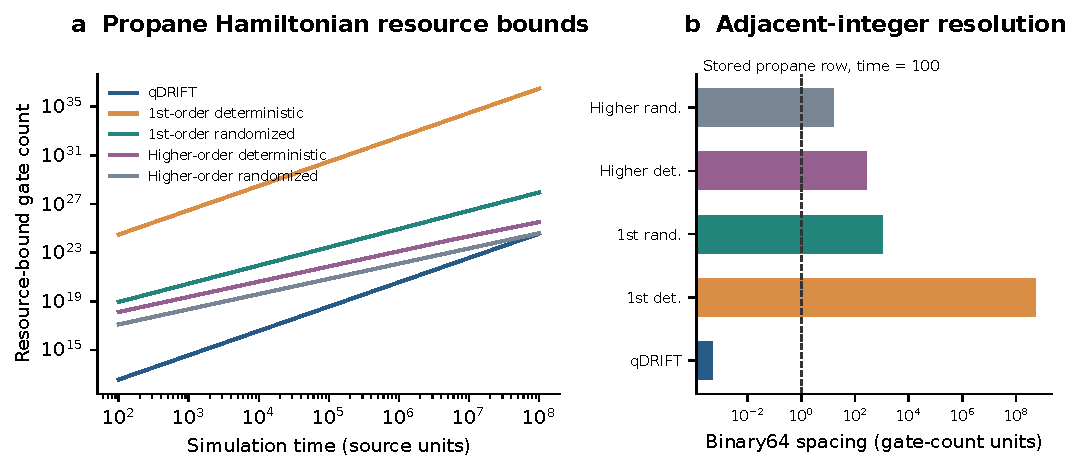
\includegraphics[width=1\linewidth,height=\textheight,keepaspectratio,alt={Resource-bound outputs and their precision requirement. a, Archived propane gate-count bounds for five compilation strategies. b, Binary64 spacing at each method's first stored propane count, at simulation time 100. The dashed line marks unit spacing; four counts cannot distinguish adjacent integers after conversion to binary64. Panel b is a new representation check on stored integers, not a rerun or independent certificate of the error-bound inequalities.}]{figures/fig2_resources.pdf}
\caption{Resource-bound outputs and their precision requirement.
\textbf{a}, Archived propane gate-count bounds for five compilation
strategies. \textbf{b}, Binary64 spacing at each method's first stored
propane count, at simulation time 100. The dashed line marks unit
spacing; four counts cannot distinguish adjacent integers after
conversion to binary64. Panel b is a new representation check on stored
integers, not a rerun or independent certificate of the error-bound
inequalities.}
\end{figure}

\subsection{Interacting quantum walks in exact particle
sectors}\label{interacting-quantum-walks-in-exact-particle-sectors}

The source target in PRAgent's quantum-walk case is the density and
correlation structure of interacting excitations. The public code
implements the coherent theoretical model associated with the
superconducting-processor experiment of Yan and colleagues {[}7{]}. A
Bose-Hubbard Hamiltonian provides the case formulation, \[
H=\sum_{j=1}^{L-1}J_j(a_j^\dagger a_{j+1}+a_{j+1}^\dagger a_j)
+\sum_{j=1}^{L}\frac{U_j}{2}n_j(n_j-1)+\sum_{j=1}^{L}h_jn_j.
\] The implementation retains source-linked coupling and interaction
parameters and works in fixed-particle-number sectors. The
one-excitation calculation uses an 11-site sector for the corresponding
source setup. The two-excitation calculation uses 12 sites, with 78
bosonic occupation states and 66 states in the hard-core limit. These
representations implement the stated theoretical sectors; they do not
reproduce the experimental hardware or its raw measurements.

The computational structure makes the physical model inspectable. The
basis is enumerated as occupation tuples, and hopping matrix elements
carry the bosonic factors \(\sqrt{n_j(n_{j+1}+1)}\). A Hermitian
eigendecomposition is reused to evaluate time evolution on the requested
grid. Observable functions then compute site density and the
two-particle correlator, \[
G_{ij}=\langle a_i^\dagger a_j^\dagger a_i a_j\rangle,
\] including the diagonal convention
\(G_{ii}=\langle n_i(n_i-1)\rangle\). The calibrated interaction,
free-boson and hard-core cases share a transparent comparison structure.

Figure 3a displays the stored one-excitation density for a central
launch. The correlation matrices in Fig. 3b--d show the calibrated
interaction and its two control models for the same two-excitation
launch and displayed time. The shared solver and observable definitions
allow a controlled comparison of how the interaction model changes the
spatial correlation pattern.

We independently recomputed the density-sum diagnostic from the stored
CSV values. Across 1,503 one-excitation state-time slices, the maximum
deviation from one is \(1.78\times10^{-15}\). Across 3,006
two-excitation slices, including the recorded model and launch
combinations, the maximum deviation from two is \(2.66\times10^{-15}\).
These residuals establish internal conservation consistency. In a
normalized fixed-number sector, the density sum equals the particle
number by construction: incorrect couplings or an incorrect comparison
time can still pass this test. It therefore supplies no quantitative
measure of agreement with the source density or correlation curves.

The supported capability is the implemented connection between physical
structure and computation: the conserved sector determines the basis,
one propagation supplies several observables, and explicit limits
provide controls. The public comparison still has an unresolved
source-time discrepancy and missing author realization-level parameters.
Until those conditions and direct observable errors are checked, this
chain establishes model implementation and internal consistency rather
than source-result reproduction.

\begin{figure}
\centering
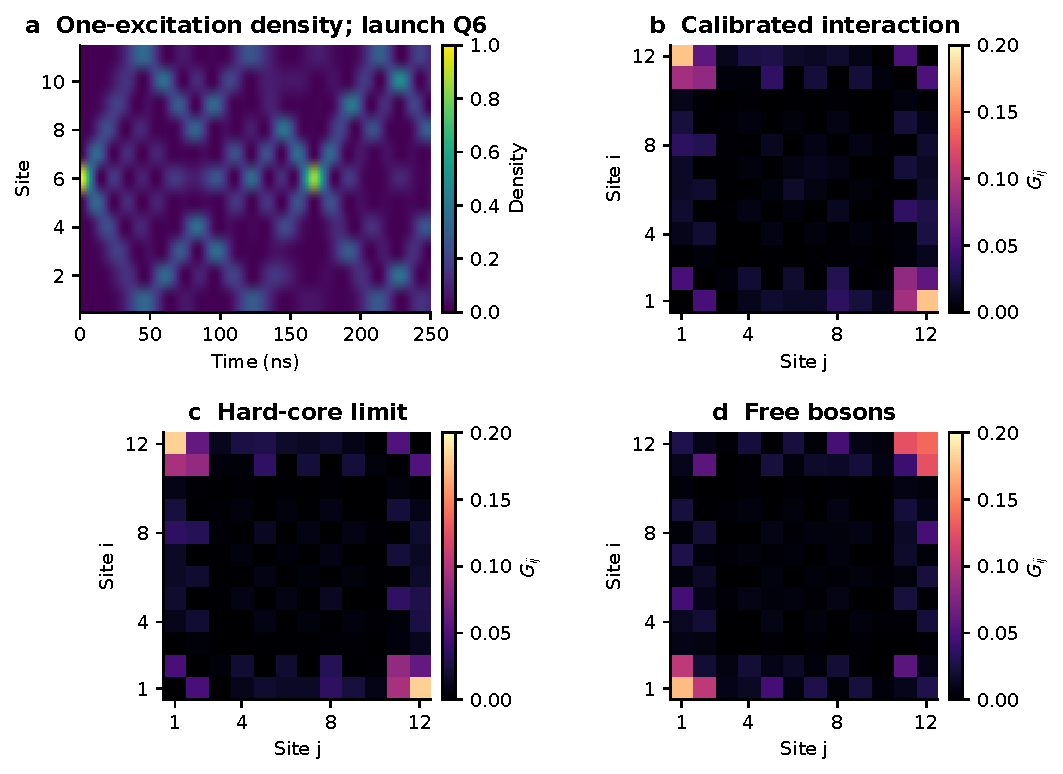
\includegraphics[width=1\linewidth,height=\textheight,keepaspectratio,alt={Quantum-walk outputs regenerated from stored arrays. a, One-excitation density after launch at site Q6 in the 11-site setup. b--d, Two-excitation correlators at 55.5 ns for launch Q6+Q7 in the 12-site setup, using calibrated interactions, the hard-core limit and free bosons. The correlation panels share a color scale. These are generated model outputs, not experimental measurements; the displayed time is taken from the archived table and is not an adjudication of the case's unresolved source-time issue.}]{figures/fig3_quantum_walks.pdf}
\caption{Quantum-walk outputs regenerated from stored arrays.
\textbf{a}, One-excitation density after launch at site Q6 in the
11-site setup. \textbf{b--d}, Two-excitation correlators at 55.5 ns for
launch Q6+Q7 in the 12-site setup, using calibrated interactions, the
hard-core limit and free bosons. The correlation panels share a color
scale. These are generated model outputs, not experimental measurements;
the displayed time is taken from the archived table and is not an
adjudication of the case's unresolved source-time issue.}
\end{figure}

\subsection{Quantum discord: separating ensembles, references and
logical
claims}\label{quantum-discord-separating-ensembles-references-and-logical-claims}

PRAgent's discord case demonstrates ensemble-based computation and
interpretation of a numerical discrepancy. It implements the DQC1
correlation problem considered by Datta, Shaji and Caves {[}8{]}. For a
unitary \(U\) acting on a register of dimension \(d\) and control
polarization \(\alpha\), the case constructs \[
\rho=\frac{1}{2d}\begin{pmatrix}I_d&\alpha U^\dagger\\\alpha U&I_d\end{pmatrix}.
\] It computes entropic quantities and measurement-dependent conditional
entropies using explicit numerical representations. The source question
motivates comparing the resulting discord with an analytical reference,
while the implementation must also specify the unitary ensemble and
optimization procedure.

The public numerical-method record describes two separately generated
ensembles of 500 matrices in \(U(32)\): a QR-based Haar construction and
a depth-32 local brickwork construction. The latter is explicitly
identified as an independent probe because the original finite
pseudorandom generator is not published. Each curve is stored on a
41-point polarization grid, with mean, standard deviation, standard
error and interval fields. This representation keeps sampling variation
visible instead of presenting an individual realization as a universal
result.

Figure 4 shows the archived means and their deviations from the
analytical reference. At \(\alpha=1\), the stored QR-Haar mean is
0.537735 bits, the brickwork mean is 0.537483 bits and the reference is
0.557305 bits. Their corresponding differences from the reference are
approximately \(-0.01957\) and \(-0.01982\) bits. The displayed bands
use the case's stored pointwise 95\% interval endpoints. They describe
ensemble uncertainty under the recorded procedure, not simultaneous
confidence bands or uncertainty in the analytical expression.

Both generators feed the same entropy and measurement-optimization
implementation. The archived production configuration specifies 129
projective axes for this shared routine. Agreement between the two
ensemble means is therefore not a comparison of independent discord
implementations. Their narrow intervals describe sampling variability
and cannot exclude shared discretization, optimization or formula
errors. The observed discrepancy is preserved in the archived outputs,
but its cause remains unresolved; finite-size effects and shared
numerical bias require discriminating checks before a physical or
source-paper conclusion follows. The demonstrated capability is
producing and exposing this comparison with its sampling conditions, not
having resolved the discrepancy.

The code also makes a useful logical distinction in its treatment of
entanglement. For the control-register split, it constructs a convex
product-state decomposition from the eigenbasis of \(U\). For other
partitions, one-sided tests such as negativity are recorded as detection
criteria. Failure to detect entanglement is not used as a separability
proof. This illustrates how the interpretation of a numerical check can
be as important as its implementation.

\begin{figure}
\centering
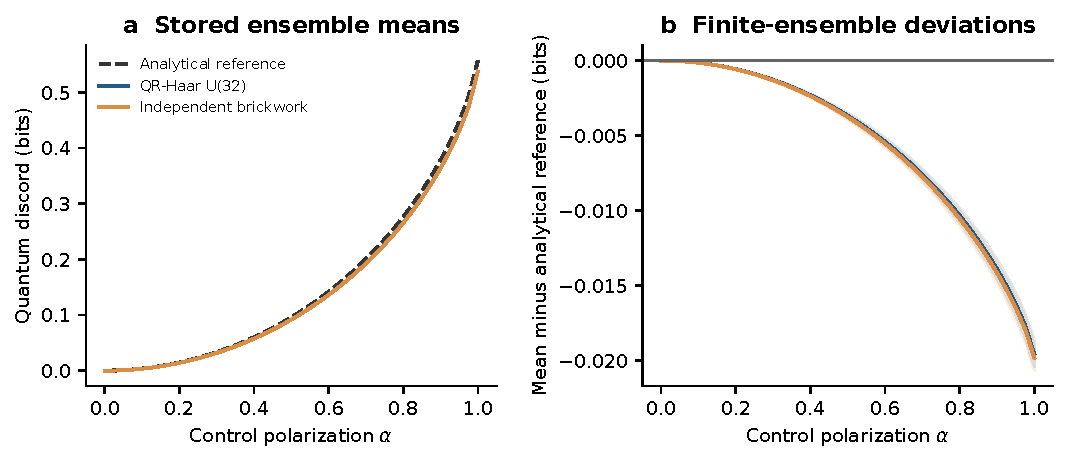
\includegraphics[width=1\linewidth,height=\textheight,keepaspectratio,alt={Quantum-discord outputs redrawn from the archived DQC1 case. a, The analytical reference and means of the QR-Haar and separately generated brickwork ensembles, evaluated through shared numerical routines. b, Mean-minus-reference residuals expose deviations that are less visible in the main curves. Shading uses the stored pointwise interval endpoints. Ensemble specifications originate in the public method record; these are generated case outputs rather than recovered author samples.}]{figures/fig4_discord.pdf}
\caption{Quantum-discord outputs redrawn from the archived DQC1 case.
\textbf{a}, The analytical reference and means of the QR-Haar and
separately generated brickwork ensembles, evaluated through shared
numerical routines. \textbf{b}, Mean-minus-reference residuals expose
deviations that are less visible in the main curves. Shading uses the
stored pointwise interval endpoints. Ensemble specifications originate
in the public method record; these are generated case outputs rather
than recovered author samples.}
\end{figure}

\section{Evidence across the 100-paper
project}\label{evidence-across-the-100-paper-project}

\subsection{Selection and source-result
linkage}\label{selection-and-source-result-linkage}

The analysis retains one fixed roster of 100 paper identities. It is a
retrospective, purposive collection rather than a preregistered
benchmark. The selection history contains 103 identities: three archived
cases were replaced after evidence limitations were identified, and
three low-compute studies were selected for planned work. The excluded
cases lacked established comparisons for NiO arrays, source-condition
rheology, or a 30-material comparison; all six identities and the
recorded reasons are preserved in
\texttt{anc/selection\_provenance.json}. This outcome-informed selection
limits population-level performance claims. The three planned studies
remain unmeasured in this snapshot; they are included in the same roster
without imputed scores.

The public extraction contains code for 97 cohort members and data for
96. To separate file availability from scientific support, we audit the
linkage of archived result objects to source references, execution
targets, declared parameter matches, reference types and cited public
files. The inventory has 3,241 object records from 95 papers. Two
further cases have assessment records but no object inventory; three
have no measurements. Objects vary in granularity, including curves and
result components, so their count is not a common scientific
denominator.

The audit identifies 950 records whose mapped targets all declare
paper-exact conditions and a numerical reference; 1,176 with a proxy,
subset or reduced-scale comparison; 675 with unspecified or other
conditions; 423 with figure or feature references; and 17 with mixed or
insufficient comparison metadata. These are descriptions of archived
evidence scope, not newly certified outcomes. In particular, the first
category does not establish that the declared conditions or numerical
comparator are correct. The accompanying object ledger preserves those
declarations, source locations, gaps and cited-file availability so that
a later scientific review can examine them individually.

\subsection{What the historical percentages
measure}\label{what-the-historical-percentages-measure}

Figure 5a--b reconstructs an archived table dated 27 August 2026. Across
97 measured papers it contains 1,399 numerical claims, 3,667 distinct
checks and 16,376 claim--check associations. Fifteen non-numerical
claims are excluded. Define \[
h_c=\frac{\#\{\text{checks associated with }c\text{ and labelled reproduced}\}}
{\#\{\text{checks associated with }c\}}.
\] Associations include supporting checks, and the same check can
contribute to several claims. The mean of \(h_c\) over claims is 40.9\%;
averaging first within each paper and then over measured papers gives
57.8\%. These are archived check-label fractions. They do not measure
the fraction of source results reproduced, the extent of agreement with
source observables, or whole-paper completion.

The metric depends on how a check list is partitioned: duplicating one
positive check can change \(h_c\) without changing a calculation or its
agreement with the paper. The ancillary sensitivity table demonstrates
this on mixed-label claims. Restricting associations to the primary
claim would still not establish direct scientific support. We retain the
historical fractions to describe the archive, and use the source-result
ledger and detailed examples to identify what evidence each calculation
actually supplies.

\subsection{Joint states and conflicting
records}\label{joint-states-and-conflicting-records}

The completion summaries mark numerical scope complete for 83 papers,
science passed for 34, and independent review passed for 26. A separate
historical set of 26 papers has \(h_c=1\) for every measured claim.
Table 2 shows that these two sets of 26 are disjoint. Furthermore, only
one paper has both summary-level science and review marked passed.
Marginal counts therefore cannot be interpreted as successive stages of
a successful reproduction funnel. Review status is also distinct from
the scientific conclusion: case \texttt{1803.01876} has review passed,
science failed and paper assessment inconclusive in both records. Thus a
passed review label cannot itself be read as a positive reproduction
certificate.

\begin{longtable}[]{@{}
  >{\raggedright\arraybackslash}p{(\linewidth - 4\tabcolsep) * \real{0.2727}}
  >{\raggedleft\arraybackslash}p{(\linewidth - 4\tabcolsep) * \real{0.3636}}
  >{\raggedleft\arraybackslash}p{(\linewidth - 4\tabcolsep) * \real{0.3636}}@{}}
\caption{Two separate contingency tables share the review columns; the
first two rows and last two rows each sum to 97. Three unavailable cases
remain outside each comparison. Case identities are supplied in the
joint-state ledger.}\tabularnewline
\toprule\noalign{}
\begin{minipage}[b]{\linewidth}\raggedright
Condition among 97 available cases
\end{minipage} & \begin{minipage}[b]{\linewidth}\raggedleft
Review passed in summary
\end{minipage} & \begin{minipage}[b]{\linewidth}\raggedleft
Review not passed in summary
\end{minipage} \\
\midrule\noalign{}
\endfirsthead
\toprule\noalign{}
\begin{minipage}[b]{\linewidth}\raggedright
Condition among 97 available cases
\end{minipage} & \begin{minipage}[b]{\linewidth}\raggedleft
Review passed in summary
\end{minipage} & \begin{minipage}[b]{\linewidth}\raggedleft
Review not passed in summary
\end{minipage} \\
\midrule\noalign{}
\endhead
\bottomrule\noalign{}
\endlastfoot
Historical check-label fraction 100\% & 0 & 26 \\
Historical check-label fraction below 100\% & 26 & 45 \\
Science passed in summary & 1 & 33 \\
Science not passed in summary & 25 & 38 \\
\end{longtable}

Even within the same frozen Git revision, summary and detailed records
disagree for six science states, six review states, seven execution
states and one numerical-scope state. Additional conflicts concern
assessment, provenance and evidence dimensions. We do not choose a
preferred label without reconciliation. Figure 5c instead shows
agreement, conflict and missingness explicitly: the two records agree on
a positive scope state for 83 papers, a positive science state for 32
and a positive review state for 26. Agreement is consistency between
records, not independent confirmation of their scientific validity.

Neither record set marks any available case complete. Among the 26
papers with all associated checks historically labelled reproduced, the
detailed records show 20 reviews missing, three stale and three passed.
They also record 22 attested executions and four missing attestations.
Other overlapping blockers include seven cases with missing parameter
provenance and five with targets not declared paper-exact. The three
review-passed cases retain mixed or paper-error-candidate assessments
and other blockers. This explains why local labels cannot establish
completion; it does not reduce all incompleteness to a lack of compute
or a single isolation-backend issue. Nor does a missing review prove
that an otherwise unexamined scientific result is wrong.

\begin{figure}
\centering
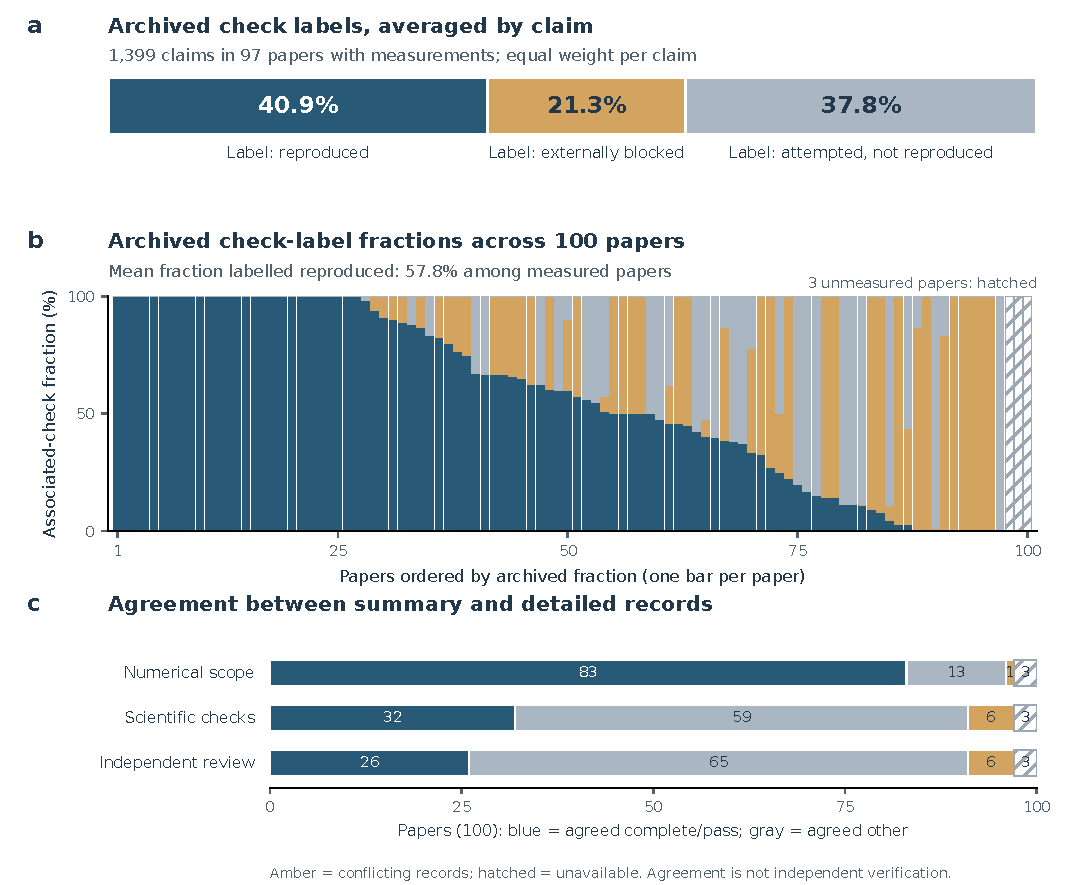
\includegraphics[width=1\linewidth,height=\textheight,keepaspectratio,alt={Historical check labels and assessment-record consistency for the fixed 100-paper project. a, Fractions of associated checks carrying each archived label, averaged over 1,399 claims. b, The same fractions by paper; hatched bars retain three unmeasured papers. The 57.8\% mean weights measured papers equally. Supporting and shared checks contribute to both panels, so neither is a scientific reproduction rate. c, Agreement between completion summaries and detailed states, with conflicts and unavailable records shown separately and a fixed denominator of 100. Agreed positive means complete scope or passed science/review in both records; it is not a new verification verdict.}]{figures/fig_overall_reproduction.pdf}
\caption{Historical check labels and assessment-record consistency for
the fixed 100-paper project. \textbf{a}, Fractions of associated checks
carrying each archived label, averaged over 1,399 claims. \textbf{b},
The same fractions by paper; hatched bars retain three unmeasured
papers. The 57.8\% mean weights measured papers equally. Supporting and
shared checks contribute to both panels, so neither is a scientific
reproduction rate. \textbf{c}, Agreement between completion summaries
and detailed states, with conflicts and unavailable records shown
separately and a fixed denominator of 100. Agreed positive means
complete scope or passed science/review in both records; it is not a new
verification verdict.}
\end{figure}

\section{Diagnostic capability and observed
obstacles}\label{diagnostic-capability-and-observed-obstacles}

PRAgent's diagnostic records connect an observed obstacle to a
discriminating test or a missing scientific requirement. Source
ambiguity, incomplete implementation, execution resources and
experimental apparatus provide four directions for investigation. The
three examples below illustrate this process without estimating cause
prevalence. The consistency audit above preserves conflicts before
diagnostic interpretation. Source pointers and recorded confidence for
the examples are supplied in \texttt{anc/obstacle\_examples.json}.

\textbf{Testing source identifiability.} For Fig. 2 of Phys. Rev.~Lett.
124, 113601 (target T001), the archived diagnosis identifies unspecified
finite-chain boundaries, site-index origin and localization conventions.
The recorded source audit and identifiability test find that
publication-compatible choices produce different energy and
inverse-participation-ratio arrays and localized-state counts. This
supports a limitation on identifying one exact numerical target from the
disclosed inputs. Resolving it requires obtaining the missing
conventions, fixing them before comparison and rerunning the
calculation. Pending gates remain in the record; the diagnosis does not
establish a false physical claim or independently exclude implementation
error.

\textbf{Checking implementation scope.} The surface-code example in
Table 1 distinguishes an incomplete scientific method from a missing
author artifact. A local proxy can be tested and executable while
failing the requested model. The required next capability is a
surface-code circuit and lifecycle-aware decoder, followed by validation
on tractable instances and evaluation of the source observable.
Additional hardware alone would not supply that missing method.

\textbf{Relating execution requirements to measurements.} Case
\texttt{1709.03478} (T002) records reduced-scale tests and one full-size
stationary block, while the complete production and convergence campaign
remains unexecuted. Its diagnosis reports 2,784 CPU tasks and 27.004229
seconds for the measured block, giving a 20.88 CPU-hour baseline before
aggregation. Finite-time tasks may take longer; the available A100 has
no validated CUDA implementation. This provides an execution estimate
for the current method, without separating resource allocation from
scheduling or backend choices. Follow-up requires an allocated CPU
campaign or a validated alternative backend, then convergence checks.

These are archived diagnostic examples, not new independent causal
verdicts. Missing data or supplementary material does not establish
missing experimental apparatus; that requires checking the physical
operations and device access. Evidence availability also limits
diagnosis: in \texttt{2506.06669}, a later pulse-definition explanation
cites a detailed test file absent from the public snapshot. That
explanation still needs inspectable support. Retaining such limits lets
the workflow specify what evidence is needed next.

\section{Capability boundaries and next evaluation
steps}\label{capability-boundaries-and-next-evaluation-steps}

The cases demonstrate different components of PRAgent's scientific work:
implementing the relevant mathematical object, handling numerical
constraints, checking physical structure and retaining evidence for
further investigation. The implementations are reusable beyond the
original interaction. A particle-sector solver, precision-aware bound
evaluator or ensemble-analysis routine can support a new calculation
when its model assumptions remain appropriate.

These capabilities were exercised within a human-guided system.
Historical model versions, interaction budgets and interventions are not
uniformly recorded, so the evidence does not isolate an autonomous
model's contribution or measure the gain over a human-only workflow. The
fixed cohort is purposively selected, and the detailed examples were
chosen with knowledge of their outputs. A controlled evaluation would
need recorded intervention and resource budgets, common acceptance
criteria and a comparison condition.

The report adds documentary re-adjudication of evidence scope and
consistency, plus arithmetic checks on selected stored arrays. It does
not independently revalidate every source comparison, execution or
causal diagnosis. A cited-file presence check establishes availability
only; it does not certify the file's scientific content. Missing public
files limit external verification even where a private run may have
existed. Later production-backend readiness is a separate deployment
issue and cannot be used to explain all archived completion states.

The next evaluation should test whether these implemented capabilities
transfer to new papers under a recorded protocol. Useful measures
include agreement with independently checked observables, correct
handling of model limits, the validity of diagnostic follow-up and the
human effort needed to complete a task. Source clarification, missing
method implementations and full-scale execution remain concrete
development priorities identified by the cases.

\section{Conclusion}\label{conclusion}

PRAgent's public cases provide concrete implementations of
precision-sensitive resource evaluation, conserved-sector quantum
dynamics and finite-ensemble discord analysis. The surface-code example
adds a system-level result: the assessment records retain a passing
proxy calculation while leaving the original target unaccepted. These
examples make the system's scientific representation, numerical methods
and acceptance distinctions inspectable. The 100-paper audit also
identifies where a broader capability claim would exceed the evidence:
auxiliary check labels are not source-result success rates, review and
science states often do not overlap, and some records conflict. The
resulting source-object ledger makes the next evaluation concrete:
verify the declared comparison conditions and numerical references,
reconcile the assessment records, and test new papers with recorded
human interventions and resource budgets.

\section*{Data, code and
reproducibility}\label{data-code-and-reproducibility}
\addcontentsline{toc}{section}{Data, code and reproducibility}

The public case archive is available at
\href{https://github.com/xi-zhao/RunThePaper/tree/43a64cd03824edb136b549f352412e8d263d9361}{RunThePaper,
revision 43a64cd}. The three implementations are identified by case IDs
\texttt{1811.08017}, \texttt{10.1126-science.aaw1611} and
\texttt{0709.0548}. The report package includes input hashes, numerical
summaries, a unified cohort roster, source-object and state-conflict
ledgers, joint-state tables and the concrete proxy assessment chain. The
accompanying analysis scripts read frozen public Git objects and
reconstruct all new numerical figures without executing case code; the
workflow schematic is retained as a conceptual diagram. The private
production environment is not included in this release.

\section*{AI assistance and manuscript
responsibility}\label{ai-assistance-and-manuscript-responsibility}
\addcontentsline{toc}{section}{AI assistance and manuscript
responsibility}

AI-assisted tools were used in software development, manuscript
preparation and the visual design of the workflow schematic. Numerical
figures were plotted from the archived arrays. The report does not
attribute authorship to an AI system or claim a uniformly autonomous
experimental campaign. The human authors are responsible for the
interpretation of results, citations and final submitted text.

\section*{References}\label{references}
\addcontentsline{toc}{section}{References}

\begingroup\small

\begin{enumerate}
\def\labelenumi{\arabic{enumi}.}
\item
  Sandve, G. K., Nekrutenko, A., Taylor, J. and Hovig, E. Ten Simple
  Rules for Reproducible Computational Research. \emph{PLoS
  Computational Biology} \textbf{9}, e1003285 (2013).
  \href{https://doi.org/10.1371/journal.pcbi.1003285}{doi:10.1371/journal.pcbi.1003285}.
\item
  Pineau, J. et al.~Improving Reproducibility in Machine Learning
  Research (A Report from the NeurIPS 2019 Reproducibility Program).
  \emph{Journal of Machine Learning Research} \textbf{22}(164), 1--20
  (2021).
  \href{https://www.jmlr.org/papers/v22/20-303.html}{jmlr.org/papers/v22/20-303.html}.
\item
  Starace, G. et al.~PaperBench: Evaluating AI's Ability to Replicate AI
  Research. \emph{arXiv} \textbf{2504.01848} (2025).
  \href{https://arxiv.org/abs/2504.01848}{arxiv.org/abs/2504.01848}.
\item
  Siegel, Z. S., Kapoor, S., Nagdir, N., Stroebl, B. and Narayanan, A.
  CORE-Bench: Fostering the Credibility of Published Research Through a
  Computational Reproducibility Agent Benchmark. \emph{arXiv}
  \textbf{2409.11363} (2024).
  \href{https://arxiv.org/abs/2409.11363}{arxiv.org/abs/2409.11363}.
\item
  Chan, J. S. et al.~MLE-bench: Evaluating Machine Learning Agents on
  Machine Learning Engineering. \emph{arXiv} \textbf{2410.07095} (2024).
  \href{https://arxiv.org/abs/2410.07095}{arxiv.org/abs/2410.07095}.
\item
  Campbell, E. A random compiler for fast Hamiltonian simulation.
  \emph{Physical Review Letters} \textbf{123}, 070503 (2019).
  \href{https://doi.org/10.1103/PhysRevLett.123.070503}{doi:10.1103/PhysRevLett.123.070503}.
  Source preprint:
  \href{https://arxiv.org/abs/1811.08017v2}{arXiv:1811.08017v2}.
\item
  Yan, Z. et al.~Strongly correlated quantum walks with a 12-qubit
  superconducting processor. \emph{Science} \textbf{364}, 753--756
  (2019).
  \href{https://doi.org/10.1126/science.aaw1611}{doi:10.1126/science.aaw1611}.
\item
  Datta, A., Shaji, A. and Caves, C. M. Quantum Discord and the Power of
  One Qubit. \emph{Physical Review Letters} \textbf{100}, 050502 (2008).
  \href{https://doi.org/10.1103/PhysRevLett.100.050502}{doi:10.1103/PhysRevLett.100.050502}.
  Source preprint:
  \href{https://arxiv.org/abs/0709.0548}{arXiv:0709.0548}.
\end{enumerate}

\endgroup

\clearpage

\section*{Supplement: unified project
roster}\label{supplement-unified-project-roster}
\addcontentsline{toc}{section}{Supplement: unified project roster}

The project retains all 100 identities in one roster. The matrix below
records evidence availability and mapping gaps, without defining
origin-based comparison groups. Blue indicates available extracted
material, amber a recorded gap, white absence within an available
extraction and gray a measurement not assessed. These indicators
describe public evidence organization, not scientific-success grades.
Full titles and the selection provenance are supplied with the
accompanying data.

\begin{center}
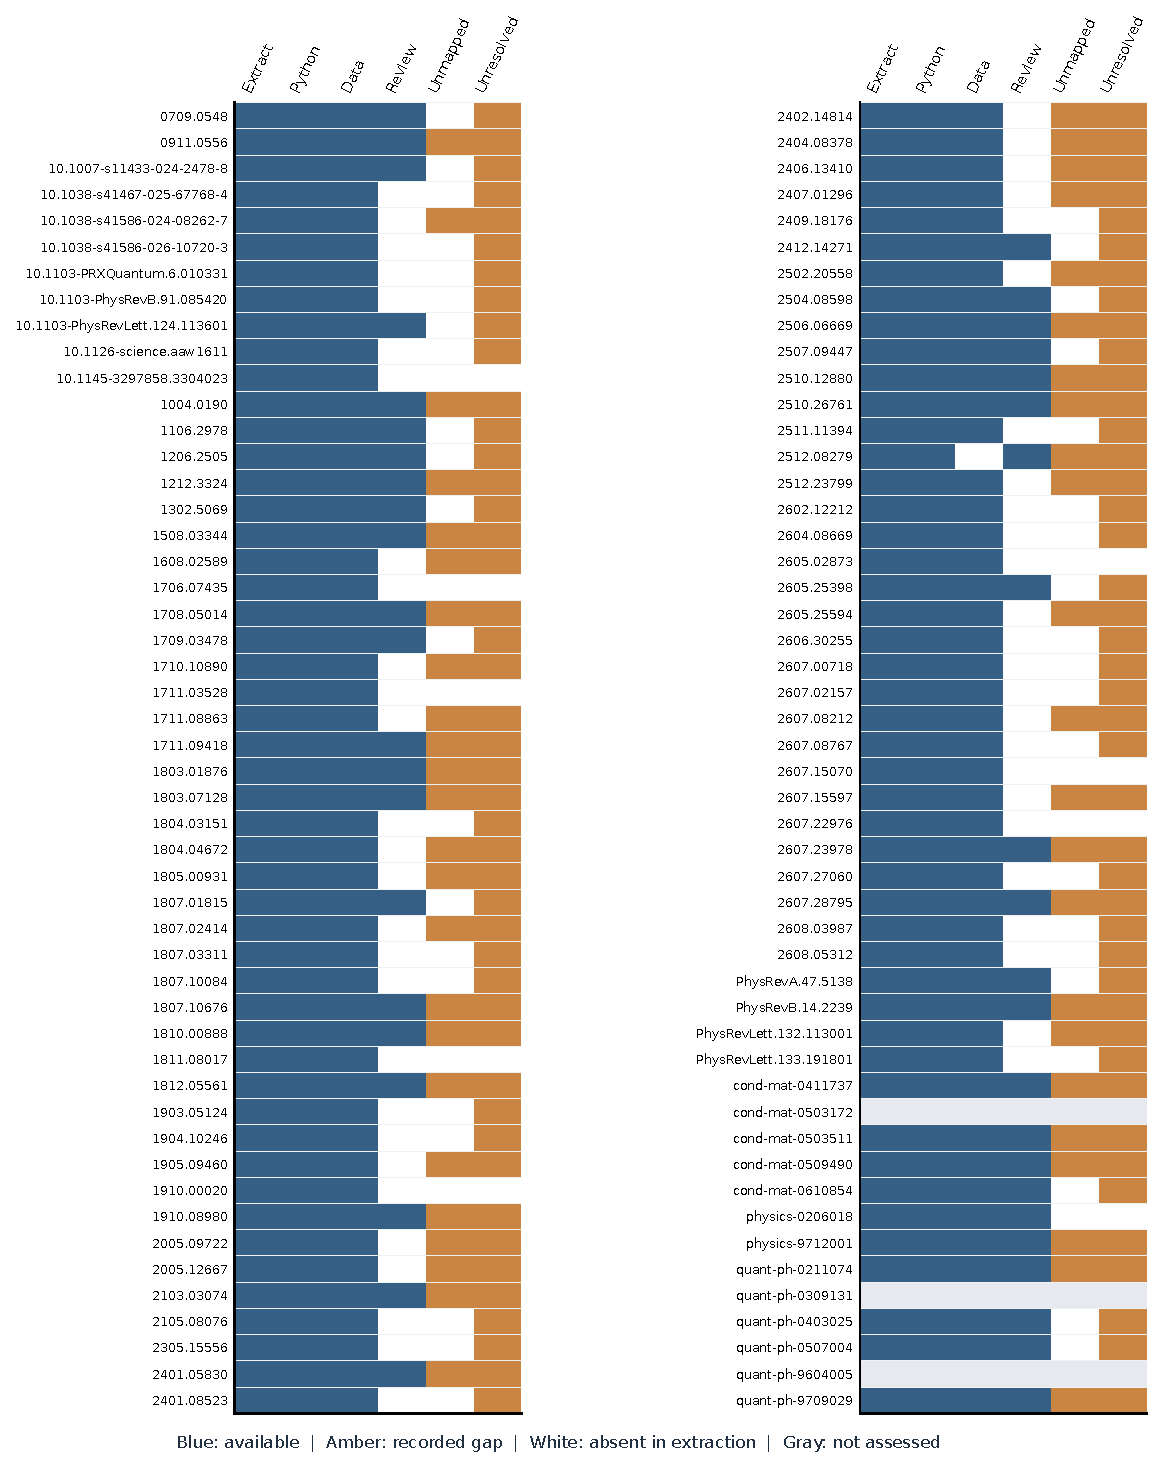
\includegraphics[width=0.94\textwidth,height=0.78\textheight,keepaspectratio]{figures/figS1_cohort_matrix.pdf}

\small\textbf{Supplementary Fig. S1.} Evidence availability for the fixed 100-paper project.
\end{center}
\end{document}
